\documentclass[fleqn,10pt]{wlscirep}
\usepackage[utf8]{inputenc}
\usepackage[T1]{fontenc}
\usepackage{float}
\usepackage{indentfirst}
\usepackage{booktabs}  % Để kẻ dòng kẻ đẹp (toprule, midrule)
\usepackage{graphicx}  % Để dùng resizebox co giãn bảng
\usepackage{array}     % Để xử lý căn chỉnh cột
\usepackage{float}     % Để dùng [H] cố định vị trí
\title{DEEP LEARNING FOR SKIN LESION SEGMENTATION: A REVIEW}

\author[]{Duy Hung BUI 202412987 and Huy Hoang VU 202412982}

%\keywords{Keyword1, Keyword2, Keyword3}

\begin{abstract}

    Computer-Aided Diagnosis (CAD) systemes for melanoma require accurate skin lesion segmentation. Over the past decade, Deep Learning (DL) models have become the standard for this problem; howerver, in order to solve artifacts and fuzzy boundaries, there must be sophisticated optimizing strategies. This review shows a comprehensive look to computational techniques, which are categorized by their optimizing objectives. Firstly, we discuss the foundational Convolutional Neural Network (CNN) developments, from structural improvement models including Improved U-Net, Fully Convolutional Network (FCN)-based U-Net, and receptive field expansion models such as Deeplab, to automated hyperparameter management with Bayesian SegNet and attention mechanism integration models like Attention Gates, CBAMSNet. Secondly, we analyze the change to global context model FAT-Net utilising Hybrid Transformers solving the disadvantage of local inductive tendency of CNNs. Finally, we evaluate the new trend of 2024: Mamba. For instance, hybrid models such as AC-MambaSeg and VM-SwimUNet have shown their capability of balancing segmentation accuracy and linear computational efficiency ($O(N)$). The review also highlights the role of Generative Adversarial Networks (GANs) in data augmentation, which provides a perspective for developing next-generation clinical diagnostic systems.

\end{abstract}
\begin{document}

\flushbottom
\maketitle
% * <john.hammersley@gmail.com> 2015-02-09T12:07:31.197Z:
%
%  Click the title above to edit the author information and abstract
%
\thispagestyle{empty}
\section*{Introduction}
    
    The skin plays a vital role as an interface between the human body and the environment, governing essential functions such as the body temperature regulation and fluid retention. In spite of the resilience, the skin is prone to a multitude of pathologies. It is estimated that there are over 3,000 distinct types of dermatological disorders, which makes skin diseases one of the most challenging health concerns worldwide. Global Cancer Statistics 2020 states that annually, fatal skin lesions claim thousands of lives \cite{GlobalCancer}. More precisely, skin cancer ranks as the third most common human malignancy, with melanoma being its most aggressive and lethal form. Epidemiological data indicates a rapid surge in melanoma incidence over the last three decades. Notably, statistical projections estimated approximately 96,480 new diagnoses in the United States in 2019 \cite{Melanoma}.

    Dermoscopy, a non-invasive imaging technique, has improved the accuracy; however, manual interpretation of dermoscopic images is labor-intensive, subjective, and dependending heavily on the clinician's expertise. Therefore, CAD systems turn out to be indispensable tools in clinical dermatology. Within the CAD pipeline, skin lesion segmentation, which is the process of accurately delineating the lesion boundary from the surrounding healthy skin, is the most critical prerequisite.
    
    Accurate recognition of melanoma is regarded as challenges due to multiple of complexities. To begin with, the low contrast between lesions and the surrounding healthy skin often creates ambiguous boundaries \cite{FCN, GAN, Deeplab}.  Secondly, high variability in patient-specific attributes, ranging from skin pigmentation and texture to lesion morphology, complicates the detection process \cite{UNet, GAN, Deeplab, Transformer}. Furthermore, image usually contains various artifacts, including body hair, reflections, air bubbles, shadows, and inconsistent illuminating conditions \cite{FCN, UNet, GAN,Transformer}. Thirdly, the scarcity of training data leads to a severe constraint on the model's generalization capability. Fourthly, the class imbalance problem, where the lesion area is smaller than the background, significantly deters segmentation performance. Notably, these aforementioned occlusions and artifacts are pervasive in standard public dermoscopic datasets. Figure 1 visually exemplifies these impediments, showing the complexity in precise boundary delineation.

        \begin{figure}[H]
        \centering
        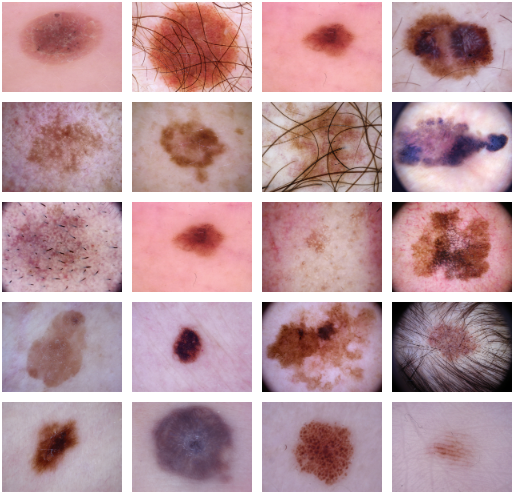
\includegraphics[width=0.8\linewidth]{ISIC2018.png}
        \caption{Dermoscopic images of some of the skin diseases from the ISIC 2016 dataset \cite{Skin}.}
        \label{fig:skindiseases}
        \end{figure}

    Early DL approaches such as FCN and U-Net, established a strong baseline but they would be struggled when there was a complex lesion heterogeneity. Consequently, recent research has moved beyond "vanilla" architectures, putting efforts on optimizing foundational models. For example, integrating structural designs (Improved U-Net), automating hyperparameter tuning (Bayesian SegNet), and evaluating attention mechanisms (Attention Gates, CBAMSNet) to enhance feature selection. Despite these solutions, CNN-based methods still remain limitation from their local receptive fields, failing to capture long-range semantic dependencies effectively.

    So as to shorten the gap, Vision Transformers (ViTs) and its hybrid models like FAT-Net were introduced, leveraging self-attention to model global context. However, quadratic computational complexity ($O(N^2)$) of ViTs has resulted in a barrier to deploy on low resource clinical devices. This trade-off has catalyzed the emergence of Mamba in 2024, offering not only the global modeling capability of Transformers but also the linear efficiency ($O(N)$) of CNNs.

    In this paper, we categorize each approach based on their optimization strategies: from data augmentation by Generative Adversarial Networks (GANs) and structural optimizations of CNNs, to the global context modeling of Transformers, and finally, the efficiency-driven era of Mamba models such as AC-MambaSeg, VM-SwinUnet. Our aim through this analysis is to identify the directions for future real-time diagnostic systems. To visualize this landscape, \textbf{Fig. \ref{fig:taxonomy}} presents the taxonomy of the computational techniques reviewed in this study.
        
        \begin{figure}[H]
            \centering
            \includegraphics[width=0.8\linewidth]{Taxonomy.jpg}
            \caption{Taxonomy of computational techniques for skin lesion segmentation utilized in this survey, categorizing methods from foundational CNNs to hybrid Mamba models.}
            \label{fig:taxonomy}
        \end{figure}

\section*{The Computational Pipeline \& Data Preparation}
    The quality of training data plays a decisive role in the performance of DL models that obey to the fundamental principle of "Garbage In, Garbage Out." particularly in dermatological analysis, the presence of artifacts and severe class imbalance necessitates sophisticated computational strategies before segmentation.

    \subsection*{Artifact Removal and Normalization}
        Artifacts such as body hair, gel bubbles, ruler markers, and uneven illumination in dermoscopic images may prevent lesion boundaries and mislead feature extraction. To deal with these issues, multiple standard pre-processing pipelines are introduced to normalize the training data. 

        Artifact Removal: Hair occlusion is the most common impediment. The DullRazor algorithm is among the standard computational approaches for the task, identifying dark hair structures using generalized grayscale morphological closing operations and subsequently replacing the occluded pixels with values interpolated from the surrounding non-occluded tissue.

        Color Normalization: Dermoscopic images are taken under different conditions of lights, color inconsistency by a wide variety of devices, preventing model convergence. Techniques such as Shades of Gray or Gray World algorithms are used to standardize the illumination and normalize the color distribution. Such methods adjust the color channels based on the average intensity, ensuring that the skin tones are consistent across the dataset.

    \subsection*{Advanced Data Augmentation Strategy via GANs}

        Class imbalance and lack of data diversity are noticing challenges in training robust skin lesion segmentation models, especially for malignant melanoma, which is always minor in public datasets. Traditional augmentation techniques, such as geometric transformations (rotation, flipping) and color jittering, are widely applied to increase the dataset size. However, these methods only produce variations of existing samples and fail to introduce sufficient diversity into the data distribution. To address the limitation, GAN has been employed as advanced data augmentation strategy. To be more precise, a GAN model consists of two competing neural networks: a Generator ($G$) and a Discriminator ($D$). $G$ tries to combine realistic lesion images from random noise distributions, while $D$ works as a binary classifier, distinguishing between real images and the synthetic ones produced by $G$. Through a min-max adversarial training process, $G$ will learn to produce excellent lesion samples capturing the complex texture and color characteristics of real dermoscopic images, which can consideralbly widen the training data.

            \begin{figure}[H]
            \centering
            \includegraphics[width=1\linewidth]{GAN.jpg}
            \caption{The flowchart of Dual Discriminator GAN architecture. After the generator module, there are two discrimination branches. One uses the concatenation of the generated mask and the original image as input, the integration is performed along the channel. The other just employs the generated mask as input.}
            \label{fig:GAN}
            \end{figure}

        Dual Discriminators by Lei et al. \cite{GAN} is an example of succeeded adversarial learning in leveraging segmentation, using $G$ for segmentation, and two distinct $D$ to supervise the results as \textbf{Fig. \ref{fig:GAN}}:

            \begin{itemize}
                \item A Global $D$ ensures the overall structural consistency of the predicted mask.
                \item A Local $D$ concentrates more on the boundary details, especially the lesion edges.
            \end{itemize}

        The system of "double scrutiny" can learns to generate not only pixel-wise accurate but also visually consistent segmentation. This study has shown the versatile potential of GANs: acting as both a tool for data augmentation and a segmentation mechanism through adversarial loss.

    \section*{Optimizing Foundational CNN Architectures}

        While early CNNs marked a noticeable change from manual feature extraction to automated learning, vanilla models often struggle with the specific challenges of dermoscopy, such as fuzzy boundaries and low contrast. Hence, the first era of advancement was defined not merely by the application of CNNs, but by the rigorous optimization of foundational architectures. This section categorizes these computational improvements into three strategic domains: structural improvement, receptive field expansion, and attention-based feature selection.

    \subsection*{Structural and Hyperparameter Optimization}

        The transition from patch-based classification to pixel-wise segmentation was pioneered by FCNs. However, the approach usually suffered from resolution loss during upsampling. To solve this, a author \cite{FCN} proposed a FCN-based model optimized with a U-Net-like architecture as \textbf{Fig. \ref{fig: FCN}}. By adapting the FCN to learn end-to-end mappings while incorporating symmetric decoding paths, the model is capable of minimizing the loss of spatial information, demonstrating that FCNs can be structurally managed to deal with quality lesion details.

            \begin{figure}[H]
                \centering
                \includegraphics[width=0.75\linewidth]{FCN.jpg}
                \caption{The flowchart of U-Net like architecture bases on FCN model.}
                \label{fig: FCN}
            \end{figure}

        Another method is to optimize the training hyperparameters. The SegNet architecture, known for its memory-efficient utilising pooling indices, is highly sensitive to parameter initialization. Sahin et al. \cite{SegNet} introduced a Bayesian Optimized SegNet which replaces manual trial-and-error by Bayesian probability. Compared with standard SegNet implementations, the model achieved superior segmentation accuracy by automatically searching for the optimal learning rate compared to standard SegNet implementations. This approach has proved that in training process, it is vital to optimize not only the architectural designs but also the computational methods.

    \subsection*{Expanding Receptive Fields via Dilated Convolutions}
            
        Standard U-Net model can be overfitting with small datasets, and limited by fixed receptive field. Liu et al. \cite{UNet} proposed an Improved U-Net \textbf{Fig. \ref{fig: UNet}} applying dialated convolution and batch normalization layer in the decoder to expand the receptive field. Therefore, the encoder-decoder path can preserve the edge information and cut down on false positives due to coarse boundary compared to the classic U-Net.

        \begin{figure}[H]
            \centering
            \includegraphics[width=1\linewidth]{UNet.jpg}
            \caption{The flowchart of Improved U-Net model with dialated convolution and batch normalization.}
            \label{fig: UNet}
        \end{figure}

        The author \cite{Deeplab} proposed a model that is the combination between RetinaNet and DeeplabV3+ named Retina-Deeplab. The RetinaNet creates sub-image normalized and centered by the lesion, and this image is segmented by the Deeplab module. Generally, the DeepLab architecture is based on a combination of Spatial Pyramid Pooling and Encoder-decoder networks architectures. DeeplabV3+ employs Atrous Spatial Pyramid Pooling to capture multi-scale context by applying dilated convolutions with varying rates in parallel and batch normalization.

    \subsection*{Feature Selection with Attention and Dynamic Mechanisms}

        As network depth increases, there are rising risks of learning redundant features (e.g., background artifacts like hair or gel), Attention Mechanisms were introduced to keep the model focused on relevant regions. Arora et al. \cite{AttentionGates} integrated Attention Gates (AGs) into the U-Net architecture. Each skip connection has a AG to distinguish feature responses in the irrelevant background regions with the high-level contextual information. By suppressing the activations in non-relevant areas, AGs enhance the model's ability to delineate fuzzy lesion boundaries, leading to better segmentation accuracy compared to standard U-Net.

        CBAMSNet \cite{CBAMSNet}, a model combined attention with dynamic computation, integrates Convolutional Block Attention Module into U-Net architecture among skip connections to refine features along both channel and spatial dimensions. The features are then extracted using stable omni-dimensional dynamic convolution, where convolutional kernels are not static but dynamically change their weights based on the input image. Therefore, it is not only lightweight and computationally efficient, but also be able to maintain the flexibility to work with the wide variety of skin lesion.

\section*{The Shift to Global Context with Hybrid Transformers}

    Although the optimized CNN architectures discussed in the previous section have considerably improved boundary delineation, each model remains disadvantages. The upsampling layer of FCN-based U-Net leads to the loss of spatial information. Improved U-Net and Deeplab models are still limited by the local nature of convolution operations, and attention-based models such as Attention U-Net and CBAMSNet are not capable of handling the context modeling limitations. Although ViTs have shown noticing advantages in various vision tasks by capturing long-range dependencies through self-attention mechanisms, these models require enormus datas to train and sometimes overlook fine-grained local details that are vital for image analysis.
    
    Therefore, the dominant strategy in medical imaging is the Hybrid Approach. A prime example is FAT-Net (Feature Adaptive Transformers) proposed by Wu et al. \cite{Transformer}, employing a Dual-Encoder Strategy contains both CNN and Transformer components with Memory-Efficient Decoder to fuse the local features and global context information extracted from the CNNs and transformer encoders. The architecture utilizes Feature Adaptive Module to adaptively activate relevant feature maps while suppressing noise. It is clear that FAT-Net outperforms pure CNN and pure Transformer models in skin lesion segmentation tasks, highlighting the effectiveness of combining local and global feature representations.

\section*{The Efficiency Revolution with State Space Models (Mamba)}
    Hybrid Transformers come with a significant computational cost when the complexity of self-attention mechanism reaches ($O(N^2)$), which is challenging to deploy on resource-constrained devices, such as mobile dermoscopy systems. In 2024, a paradigm shift occurred with the emergence of State Space Models (SSMs), specifically the Mamba architecture, which offers the global modeling capability of Transformers with linear computational complexity ($O(N)$).
       
    AC-MambaSeg \cite{Mamba}, representing the synthesis between the flexibility of CNN and the efficiency of Mamba, has replaced heavy convolution layers with Visual State Space blocks. These blocks can flatten input image in four directions, then capture the global context without the complexity of ($O(N^2)$). The efficiency is integrated by utilizing AGs and Selective Kernel modules, balancing the lite model with high speed and accuracy.

    Another hybrid model designed for segmentation tasks is VM-SwinUnet \cite{VM-SwinUnet}. While Swin Transformer blocks work on feature extraction, Visual State Space blocks deal with boundary continuity, the model shows high performance on skin lesion and retinal vessels.

\section*{Discussion \& Comparative Analysis}
    
    Models like FCN-based and Improved U-Net concentrates on the solutions to local inductive bias of convolutions through structural addition such as dilated convolutions. While these methods succeed in boundary detection, they are not able to recognize large-scale patterns or separating complex artifacts from the skin lesions. Therefore, the application of Attention Mechanisms and Transformers has marked a transition towards the context awareness of skin segmentation. However, high accuracy comes with the cost of computational complexity up to $O(N^2)$, leading to the fact that many Hybrid Transformer models are unsuitable for real-time clinical usage. The emergence of Mamba architectures in 2024 represents a enormous breakthrough. By achieving global visualization with only linear complexity ($O(N)$), Mamba hybrids are capable of addressing the trade-off between precision and speed, paving the way for lightweight, mobile-compatible diagnostic systems, shown in \textbf{Table \ref{tab:pros_cons}}.   

    \begin{table}[H]
        \centering
        \caption{Comparison of Deep Learning Architectures for Skin Lesion Segmentation: Optimization Strategies.}
        \label{tab:pros_cons}
        \resizebox{\textwidth}{!}{%
        \begin{tabular}{|p{1.75cm}|p{2.75cm}|p{5.25cm}|p{5.25cm}|}
        \hline
        \textbf{Model Family} & \textbf{Core Technique} & \textbf{Pros (Strengths)} & \textbf{Cons (Limitations)} \\ 
        \hline
        \textbf{FCN-based U-Net} \newline \cite{FCN} & End-to-End FCN + U-Net & 
        Lightweight computation and direct pixel-to-pixel learning from raw images. & 
        Local view and may produce coarse boundaries without refinement steps. \\ 
        \hline
        \textbf{Adversarial CNNs (GANs)} \newline \cite{GAN} & Dual Discriminators (Global \& Local) & 
        Solves data scarcity with synthesis and Adversarial loss enforces sharp boundaries through double scrutiny. & 
        Hard to converge and risk of hallucinating artifacts in synthesized images. \\ 
        \hline
        \textbf{Improved U-Net} \newline \cite{UNet} & Dilated Convolution + Batch Norm & 
        Expands receptive field without resolution loss and ensures a more stable training process. & 
        Lacks of true global context modeling and struggles with large or irregular lesions. \\ 
        \hline
        \textbf{Retina-DeepLab} \newline \cite{Deeplab} & Detection-driven + Graph refinement & 
        Coarse-to-fine strategy removes background noise efficiently. &
        Dependends on the accuracy of the detection step. \\ 
        \hline
        \textbf{Attention CNNs} \newline \cite{CBAMSNet} & Attention Gates / CBAM + ODConv & 
        Automatically suppresses artifacts (hair, gel) and is lightweight and adaptive to variable lesion shapes. & 
        Constrained by the static nature of convolutions and performance depends on attention map quality. \\ 
        \hline
        \textbf{Hybrid Transformer} \newline \cite{Transformer} & Dual Encoder (CNN + ViT) & 
        Captures long-range semantic dependencies (Global Context) and is robust against texture variations. & 
        Quadratic computational complexity $O(N^2)$ and requires massive data to generalize. \\ 
        \hline
        \textbf{Hybrid Mamba} \newline \cite{Mamba} & State Space Models (Selective Scan) & 
        Linear complexity $O(N)$ allows fast and balances global modeling with local CNN features. & 
        Newer architecture with less community support and potential information loss in very long sequences. \\ 
        \hline
        \end{tabular}%
        }
    \end{table}

\section*{Conclusion}
    
    The review shows the recent optimized computational techniques for skin lesion segmentation and categorizes them into enhancing objectives. We analyze how GAN architecture solves the scarcity of training data, how refined CNN addresses local contextual learning, and how hybrid ViT bridges the global context gap. Finally, we present the breakthrough of hybrid Mamba models achieving both linear complexity and impressive accuracy. In conclusion, the future of skin lesion segmentation will depend on hybrid architectures, which leverage the gold model U-Net the little complexity and high speed of Mamba, the precision of ViTs and the localized concentration of AG to generate real time, clinically reliable diagnoses.

\bibliography{sample}

\end{document}